\part{Sicurezza fisica e del personale}
\label{SFDP}
\chapter{Sicurezza fisica}

La difesa in profondità serve per proteggersi quando un livello di sicurezza
viene superato. Questo tipo di difesa è possibile immaginarsela come gli strati
di una cipolla.

È importante attrezzarsi anche per difendersi da eventi che possono accadere
all'interno dell'azienda (es. incendio).

\section{Tipologie di controlli}

Le diverse tipologie di controlli sono concentriche, a difficoltà incrementale e
indipendenti. Questi tipi di controlli possono essere \textbf{preventivi},
\textbf{reattivi} e \textbf{correttivi}.

Una lista di controlli (a partire dalla parte centrale per muoversi
verso quella più esterna) sono:

\begin{itemize}
\item Postazione di lavoro chiusa;
\item Videocamere e sistema di allarme;
\item Restrizione del personale d'accesso;
\item Guardie di sicurezza, log manuale e badge con foto identificative;
\item Singolo punto di accesso controllato e finestre sbarrate;
\item Non pubblicizzare l'ubicazione di strutture (\textit{facilities})
sensibili.
\end{itemize}

Un buon consiglio è avere un numero di accessi al locale ridotto. Questo però
non è sempre possibile, in quanto in una \textit{facility} grossa potrebbero
esserci norme di sicurezza da seguire.

Anche dal punto di vista del riconoscimento una buona pratica è
far indossare il badge al personale.

Ognuna delle misure esposte prima hanno un costo che di solito è grande, che
può portare a problemi (es. le registrazioni dovrebbero essere
salvate anche in postazioni sicure in quanto potrebbero essere soggette a furti).

Quanto spenderci e quanto investire è una questione a cui è difficile
rispondere.

\section{Sicurezza fisica}
\label{SFDP:fisica}
\subsection{Protezione dalla corrente}

Classificazione in funzione del fenomeno negativo che si verifica:
\begin{itemize}
\item \textbf{Surge, spikes and sags:} qualcuno ha collegato un dispositivo alla rete che
ha causato un sovraccarico, causando picchi (positivi e negativi);
\item \textbf{Blackout};
\item \textbf{Brownout:} i livelli di corrente dichiarati non sono quelli effettivi sulla
rete;
\item \textbf{EMI (Electromagnetic Interference):} dispositivi elettrici che generano
effetti parassitari su dispositivi terzi.
\end{itemize}

I dispositivi di protezione dipendono dalla durata del fenomeno: per la breve
durata bastano i surge protector, per durata minore di 30 min si utilizza un UPS
(universal power supply); per periodi più lunghi si usa un generatore
alternativo di corrente. I generatori possono arrivare anche a costare milioni
di euro.

\subsection{Equipaggiamento della computer room}

\begin{itemize}
\item Rilevatore d'acqua (a livello del pavimento);
\item Estintori;
\item Allarme antincendio manuale;
\item Rilevatori di fumo (in alto e in basso);
\item Interruttori di spegnimento d'emergenza.
\end{itemize}

\subsection[Ambiente IPF]{Ambiente IPF\protect\footnote{\textit{Information
processing facility}}}

È buona norma posizionare la sala di calcolo nei piani medi
dell'edificio, perché ai piani alti potrebbe essere soggetta alle
intemperie mentre nei piani inferiori potrebbe correre il rischio
di allagarsi.
Il rischio incendi deve essere mitigato pertanto è necessario
che i pompieri ispezionino l'IPF ogni anno e che l'IPF disponga
di porte tagliafuoco e muri resistenti almeno due ore in
caso di incendio.
Devono inoltre essere presenti un interruttore di emergenza con un
pannello sia dentro che fuori dalla sala di calcolo, uno scaricatore di 
tensione e un UPS.
In ultima istanza deve essere vietato fumare, bere e mangiare nell'IPF.

È compito dell'auditor richiedere la documentazione e osservare.
L'auditor può inoltre testare le batterie e gli estintori manuali.

\subsubsection{Sistema per la soppressione dei fuochi}

Questi sistemi possono essere:
\begin{itemize}
\item Acqua;
\begin{itemize}
\item Caricato: ovvero gli estintori sono caricati e hanno l'attivazione
immediata. Lo svantaggio è che essendo sempre caricati potrebbero costituire un
problema;
\item Secchi.
\end{itemize}
\item Gas;
\begin{itemize}
\item Pericolosi (che possono essere Halon e Anidride Carbonica);
\item Amici dell'ambiente, che non spengono veramente il fuoco ma riducono le
capacità ignifughe (FM-200 e Argonite).
\end{itemize}
\end{itemize}

\subsection{Sistemi di chiusura}

Esistono diverse modalità di chiusura dei sistemi, che per essere sbloccati
possono richiedere dalla autenticazione biometrica fino ad una semplice
porta elettronica.

Molti di questi sistemi sono elettrici ed è quindi importante che i
meccanismi siano \textit{fail-safe}: ovvero che in mancanza della corrente
elettrica la porta debba rimanere aperta. Proprio per questo gli attaccanti
potrebbero sfruttare ciò per guadagnare l'accesso.

\subsubsection{Porta dell'uomo morto (Deadman door)}
Questa tecnica prevede di avere due porte per controllare l'accesso.
Può essere aperta solamente una porta alla volta.
Nell'area tra le due porte può accedere \emph{una sola} persona per
volta, così viene ridotto il rischio di \textit{piggybacking}, 
cioè che una persona non autorizzata segua una autorizzata. 
È un sistema utilizzato, per esempio, dalle banche.


\subsection{Computer nei luoghi pubblici}

Protezioni logiche: Imaged computers, antivirus e antispyware, filtri web,
login/password e protezione firewall dal resto dell'organizzazione.

Protezioni fisiche: lucchetto sul case, dispositivo della kensington per i
laptop. Anche le etichette con il codice è meglio inciderle nello chassis del
laptop piuttosto che usare un'etichetta rimovibile.

\subsection{Mobile computing}

\begin{itemize}
\item Incisione del numero seriale sul laptop;
\item Backup dei dati critici e sensibili;
\item Criptare i dati sensibili;
\item Proteggere i file importanti con password individuali;
\item Individuare il responsabile del furto e segnalarlo.
\end{itemize}


\subsection{Sicurezza dei dispositivi}

Le porte USB e le entrate Flash devono essere bandite o disabilitate dal
computer. In alternativa è necessario eseguire una crittografia di tutti i dati.


\subsection{Tabella delle criticità}

\begin{figure}[H]
 \centering
 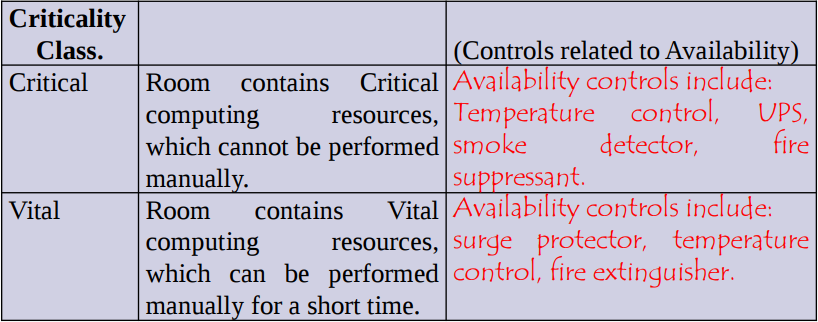
\includegraphics[width=0.8\textwidth]{criticality-table}
\end{figure}

\subsection{Mappa della sicurezza fisica}
\begin{figure}[H]
 \centering
 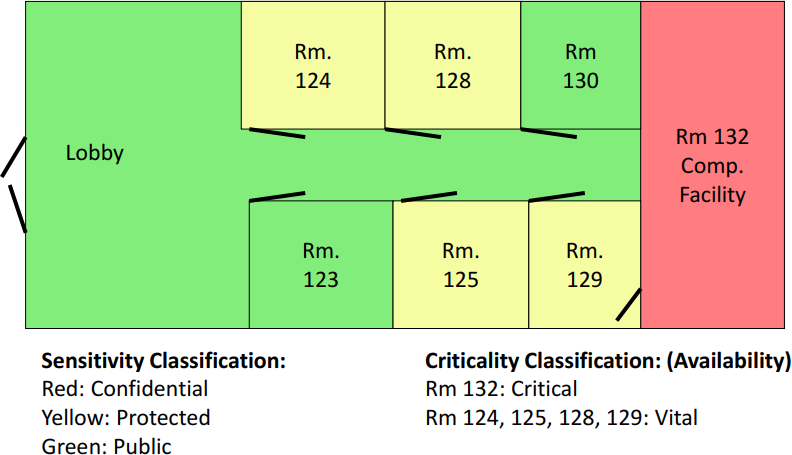
\includegraphics[width=0.8\textwidth]{physical-security-map}
\end{figure}

\subsection{Esercizi}

Gli esercizi sono disponibili nella Sezione \ref{esSFDP:fisica}.

\section{Sicurezza del personale}
\label{SFDP:DP}

\subsection{Consapevolezza della sicurezza \& Training}

Il training copre quello che ci si aspetta dagli impiegati?

Il training può essere implementato come: orientamento dei nuovi impiegati e
newsletter interna alla compagnia. Inoltre è possibile determinare l'efficacia
intervistando gli impiegati.


\subsubsection{Awareness Function: tipi di addestramento sulla sicurezza}

\textbf{Awareness:} crea nel personale una sensibilità nei confronti di problemi di
sicurezza.\\
\newline
\textbf{Training:} skill necessarie per una posizione particolare.\\
\newline
\textbf{Education:} skills di alto livello.\\
